\subsection{Izračun krivulj}
Za vsako krivuljo bom izračunal kakšna naj bi bila, glede na 
željene parametre, nato pa izbral najbližjo standardno krivuljo, 
katero lahko najdem katalogu standardnih krivulj. 
Čas enega cikla, se pravi enkraten obrat krivuljne gredi, bo 10s.
Formule bom uporabil iz poglavja \nameref{izracun_krivulj}
    
    \subsubsection{Struženje prvega in drugega roba}
        Vrtljaji: 2000 \( \frac{vrt}{min} \) \\
        Pomik: 0.04 \( \frac{mm}{vrt} \) \\
        Dolžina struženja: 1 mm

        \begin{equation}
            \begin{split}
                N &= \frac{1mm}{0.04\frac{mm}{vrt}} = 25 vrt \\
                t &= \frac{60s * 25vrt}{2000vrt} = 0.75 s \\
                \alpha &= \frac{360 \degree}{10 s} * 0.75s = 27 \degree \\
            \end{split}
        \end{equation}

        Spodaj na sliki \ref{shema_robov} sem še narisal skico orodja
        in obdelovanca pri pobiranju robov.

        \begin{figure}[H]
            \begin{center}
                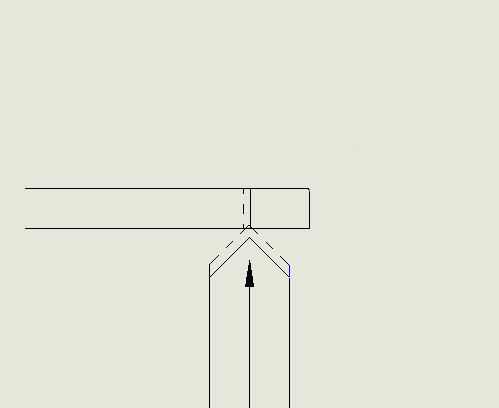
\includegraphics[width=8cm]{robi.png}
                \caption{Skica poteka pobiranja robov
                \cite{lasten}}
                \label{shema_robov}
            \end{center}
        \end{figure}

        \newpage
    
    \subsubsection{Centriranje}
        Vrtljaji: 2000 \( \frac{vrt}{min} \) + 2200 \( \frac{vrt}{min} \)\\
        Pomik: 0.03 \( \frac{mm}{vrt} \) \\
        Dolžina vrtanja: 2 mm
        
        \noindent Enako krivuljo sem uporabil tudi za povrtavanje luknje iz druge strani.

        \begin{equation}
            \begin{split}
                N &= \frac{2 mm}{0.03 \frac{mm}{vrt}} = 66.67 vrt \\
                t &= \frac{60 s * 66.67 vrt}{4200 vrt} = 0.95 s \\
                \alpha &= \frac{360\degree}{10 s} * 0.95 s = 34.2 \degree \\
            \end{split}
        \end{equation}

        Spodaj na sliki \ref{centriranje} je prikazan potek
        centriranja pred vrtanjem.

        \begin{figure}[H]
            \begin{center}
                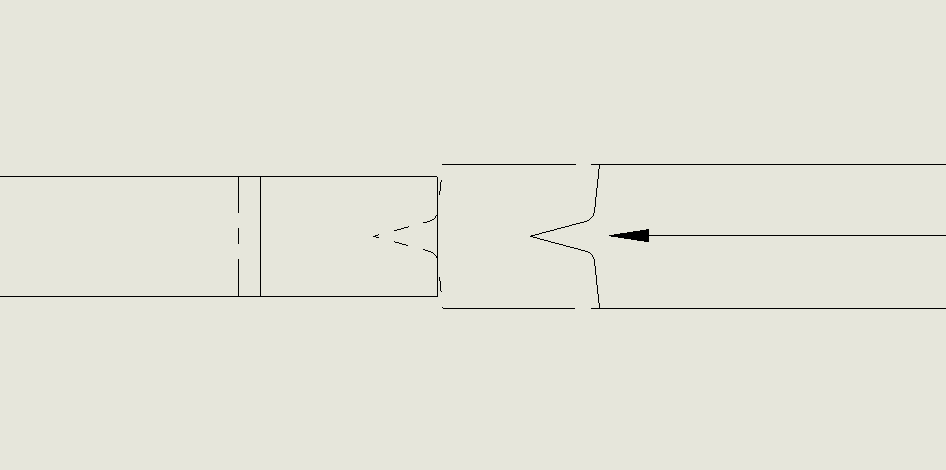
\includegraphics[width=8cm]{centriranje.png}
                \caption{Skica poteka centriranja
                \cite{lasten}}
                \label{centriranje}
            \end{center}
        \end{figure}

        \newpage

    \subsubsection{Vrtanje}
        Vrtljaji: 2000 \( \frac{vrt}{min} \) + 2200 \( \frac{vrt}{min} \)\\
        Pomik: 0.03 \( \frac{mm}{vrt} \) \\
        Dolžina vrtanja: 8 mm

        \begin{equation}
            \begin{split}
                N &= \frac{8 mm}{0.03 \frac{mm}{vrt}} = 266.67 vrt \\
                t &= \frac{60 s * 266.67 vrt}{4200 vrt} = 3.8 s \\
                \alpha &= \frac{360\degree}{10 s} * 3.8 s = 136.8 \degree \\
            \end{split}
        \end{equation}

        Na spodnji sliki \ref{vrtanje} je prikazana skica vrtanja
        luknje $\phi 1.4$.
        \begin{figure}[H]
            \begin{center}
                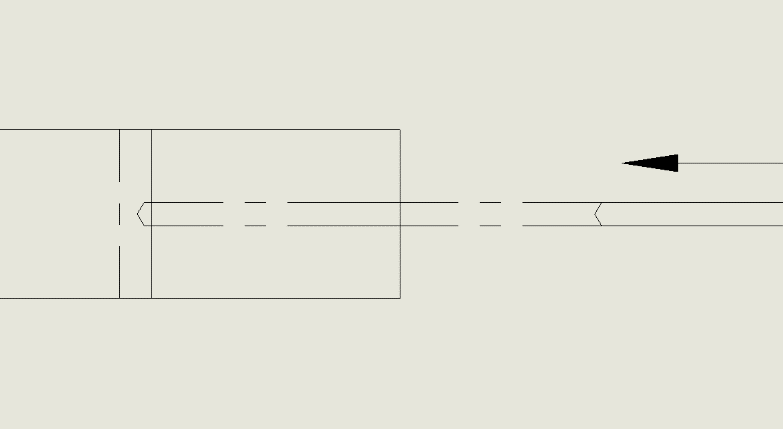
\includegraphics[width=8cm]{vrtanje.png}
                \caption{Skica poteka vrtanja
                \cite{lasten}}
                \label{vrtanje}
            \end{center}
        \end{figure}

        Zaradi večje globine vrtanja in malega premera svedra, 
        sem v krivuljo dodal luknjo zato, da se sveder očisti.
        Za premik svedrov se na tem stroju uporablja bobnaste krivulje,
        zato sem tukaj skiciral raztegnjeno bobnasto krvuljo kot prikazano
        na sliki \ref{raztegnjen_boben}. To sem kasneje
        izrezal in ovil okoli surovca in jo po črti izrezal..
        
        \begin{figure}[H]
            \begin{center}
                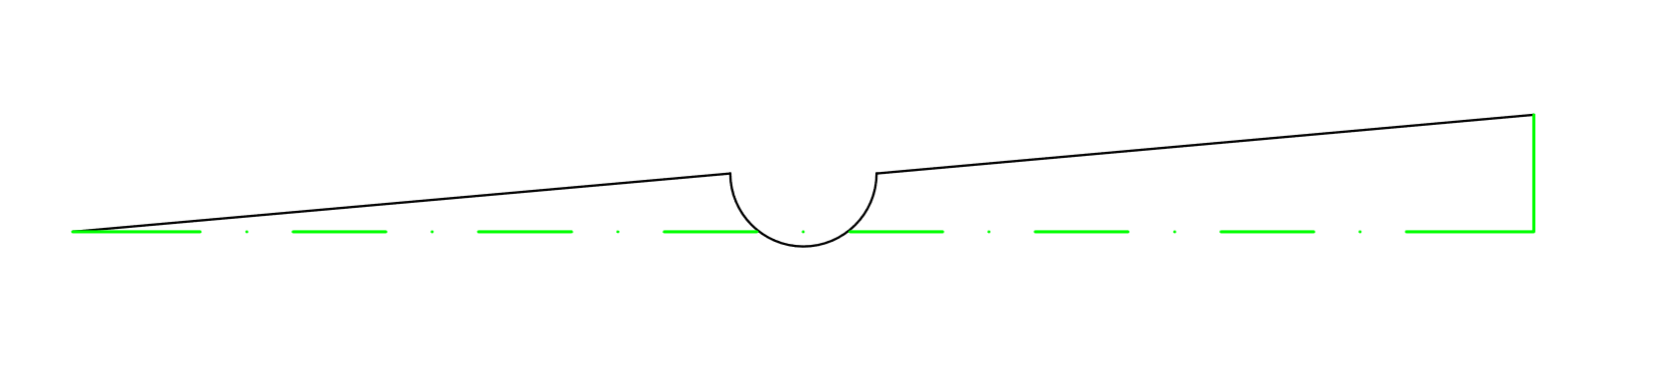
\includegraphics[width=\linewidth]{skica_krivulje_vrtanja.png}
                \caption{Raztegnjena bobnasta krivulja
                \cite{lasten}}
                \label{raztegnjen_boben}
            \end{center}
        \end{figure}
        \newpage

    \subsubsection{Odrez}
        Vrtljaji: 2000 \( \frac{vrt}{min} \) \\
        Pomik: 0.02 \( \frac{mm}{vrt} \) \\
        Dolžina struženja: 3 mm

        \begin{equation}
            \begin{split}
                N &= \frac{3mm}{0.02\frac{mm}{vrt}} = 150 vrt \\
                t &= \frac{60s * 150 vrt}{2000 vrt} = 4.5 s \\
                \alpha &= \frac{360 \degree}{10 s} * 4.5 s = 146 \degree \\
            \end{split}
        \end{equation}

        Spodaj na sliki \ref{odrez} je prikazana skica odreza kosa.
        \begin{figure}[H]
            \begin{center}
                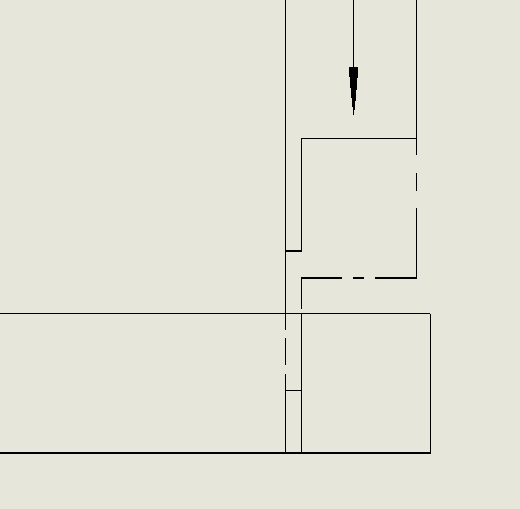
\includegraphics[width=8cm]{odrez.png}
                \caption{Skica poteka odreza
                \cite{lasten}}
                \label{odrez}
            \end{center}
        \end{figure}

        \newpage

    \subsubsection{Rezultati izračunov}
        V spodnji tabeli \ref{Tabela rezultatov} so prikazani
        rezultati mojih izračunov.
        
        \begin{table}[H]
            \caption{Tabela povzetkov izračunov krivulj}
            \label{Tabela rezultatov}
            \begin{center}
                \begin{tabular}{|c|c|c|c|}
                    \hline
                    Št. & Operacija & Vzpon [mm] & Kot [°] \\
                    \hline
                    1 & Struženje prvega roba & 1 & 27 \\
                    \hline
                    2 & Struženje drugega roba & 1 & 27 \\
                    \hline
                    3 & Centriranje & 2 & 34.2 \\
                    \hline
                    4 & Vrtanje & 8 & 136.8 \\
                    \hline
                    5 & Odrez & 3 & 146 \\
                    \hline
                \end{tabular}
            \end{center}
        \end{table}
